% This is samplepaper.tex, a sample chapter demonstrating the
% LLNCS macro package for Springer Computer Science proceedings;
% Version 2.20 of 2017/10/04
%
\documentclass[runningheads]{llncs}
%
\usepackage{graphicx,color}
\usepackage{dirtree}
%\usepackage{natbib}

\newcommand{\attribute}[1]{\texttt{#1}}
\newcommand{\topicname}[1]{\textit{#1}}
\newcommand{\componentname}[1]{\texttt{#1}}
\newcommand{\mongoname}[1]{\texttt{#1}}
\usepackage{listings}
\usepackage[colorinlistoftodos]{todonotes}
\usepackage[hidelinks]{hyperref}
\usepackage[capitalise,nameinlink]{cleveref}
\usepackage{float}

\lstdefinelanguage{PDDL}
{
  sensitive=false,    % not case-sensitive
  morecomment=[l]{;}, % line comment
  alsoletter={:,-},   % consider extra characters
  otherkeywords={-},
  morekeywords={
    define,domain,problem,not,and,or,when,forall,exists,either,
    :domain,:requirements,:types,:objects,:constants,
    :predicates,:action,:parameters,:precondition,:effect,
    :fluents,:primary-effect,:side-effect,:init,:goal,
    :strips,:adl,:equality,:typing,:conditional-effects,
    :negative-preconditions,:disjunctive-preconditions,
    :existential-preconditions,:universal-preconditions,:quantified-preconditions,
    :functions,assign,increase,decrease,scale-up,scale-down,
    :metric,minimize,maximize,
    :durative-actions,:duration-inequalities,:continuous-effects,
    :durative-action,:duration,:condition
  },
  keywordstyle = \color{blue},
}
%%
\usepackage{ifthen}
\usepackage[a4paper, total={6in, 8in}]{geometry}
\usepackage{url}
\usepackage{listings}
\usepackage{verbatim}

%% caption less table to specify restful primitives
\newcommand{\restful}[1]
{
\begin{center}
\begin{tabular}{l p{12cm}}
\hline
#1
\hline
\end{tabular}
\end{center}
\vspace{6pt}
}


%% caption less table to specify restful uri
\newcommand{\routes}[2]
{
\begin{center}
\begin{tabular}{p{\textwidth}}
\hline
\url{#1}  \\
#2
\hline
\end{tabular}
\end{center}
\vspace{6pt}
}
%
%
%
  
\newcommand{\mimetype}[2]{#1 & #2 \\\noalign{\smallskip}}
\newcommand{\head}[2]{#1 & #2 \\\noalign{\smallskip}}
\newcommand{\uri}[2]{\url{#1} \\ #2 \vspace{8pt} \\\noalign{\smallskip}}
\newcommand{\env}[2]{#1 & #2 \\\noalign{\smallskip}}
%

%%% resource definition table
\newcommand{\resource}[1]
{
\begin{center}
\begin{tabular}{l l p{12cm}}
\hline
#1
\hline
\end{tabular}
\end{center}
\vspace{6pt}
}
\newcommand{\attr}[3]{{\tt #1} & #2 & #3 \\\noalign{\smallskip}}

%
%
\newcommand{\request}[6]
{
\begin{center}
\begin{tabular}{l p{12cm}}
\hline
Synopsis:  & #1 \url{#2} \\\noalign{\smallskip}
           & #3     \vspace{4pt}\\
\ifx&#4&%
   % is empty
\else
  Precondition:  & #4 \vspace{4pt}\\
\fi
\ifx&#5&%
   % is empty
\else
  Postcondition: & #5 \vspace{4pt}\\
\fi
Status code:   & #6 \\
\hline
\end{tabular}
\end{center}
\vspace{6pt}
}

\newcommand{\method}[2]
{

\begin{center}
\begin{tabular}{l p{12cm}}
#1 \\\noalign{\smallskip}
\hline
#2
\hline
\end{tabular}
\end{center}
\vspace{6pt}
}

\newcommand{\desc}[1]
{
Description:  & #1     \vspace{4pt}\\
}

\newcommand{\precond}[1]
{
Precondition:  & #1 \vspace{4pt}\\
}

\newcommand{\postcond}[1]
{
Postcondition:  & #1 \vspace{4pt}\\
}

\newcommand{\statuscodes}[1]
{
Status code:   & #1 \\
}

\newcommand{\body}[1]
{
Body:   & \begin{minipage}{3in}\begin{verbatim}#1\end{verbatim}\end{minipage} \vspace{4pt}\\
}


\newcommand{\sep}{\\\noalign{\smallskip} &}

\newcommand{\status}[1]
{
\ifthenelse{\equal{#1}{100}}{100 Continue}{}%
\ifthenelse{\equal{#1}{101}}{101 Switching Protocols}{}%
\ifthenelse{\equal{#1}{200}}{200 OK}{}%
\ifthenelse{\equal{#1}{201}}{201 Created}{}%
\ifthenelse{\equal{#1}{202}}{202 Accepted}{}%
\ifthenelse{\equal{#1}{203}}{203 Non-Authoritative Information}{}%
\ifthenelse{\equal{#1}{204}}{204 No Content}{}%
\ifthenelse{\equal{#1}{205}}{205 Reset Content}{}%
\ifthenelse{\equal{#1}{206}}{206 Partial Content}{}%
\ifthenelse{\equal{#1}{300}}{300 Multiple Choices}{}%
\ifthenelse{\equal{#1}{301}}{301 Moved Permanently}{}%
\ifthenelse{\equal{#1}{302}}{302 Found}{}%
\ifthenelse{\equal{#1}{303}}{303 See Other}{}%
\ifthenelse{\equal{#1}{304}}{304 Not Modified}{}%
\ifthenelse{\equal{#1}{307}}{307 Temporary Redirect}{}%
\ifthenelse{\equal{#1}{302}}{302 Found}{}%
\ifthenelse{\equal{#1}{400}}{400 Bad Request}{}%
\ifthenelse{\equal{#1}{401}}{401 Unauthorized}{}%
\ifthenelse{\equal{#1}{402}}{402 Payment Required}{}%
\ifthenelse{\equal{#1}{403}}{403 Forbidden}{}%
\ifthenelse{\equal{#1}{404}}{404 Not Found}{}%
\ifthenelse{\equal{#1}{405}}{405 Method Not Allowed}{}%
\ifthenelse{\equal{#1}{406}}{406 Not Acceptable}{}%
\ifthenelse{\equal{#1}{407}}{407 Proxy Authentication Required}{}%
\ifthenelse{\equal{#1}{408}}{408 Request Timeout}{}%
\ifthenelse{\equal{#1}{409}}{409 Conflict}{}%
\ifthenelse{\equal{#1}{410}}{410 Gone}{}%
\ifthenelse{\equal{#1}{411}}{411 Length Required}{}%
\ifthenelse{\equal{#1}{412}}{412 Precondition Failed}{}%
\ifthenelse{\equal{#1}{413}}{413 Request Entity Too Large}{}%
\ifthenelse{\equal{#1}{414}}{414 Request-URI Too Long}{}%
\ifthenelse{\equal{#1}{415}}{415 Unsupported Media Type}{}%
\ifthenelse{\equal{#1}{416}}{416 Requested Range Not Satisfiable}{}%
\ifthenelse{\equal{#1}{417}}{417 Expectation Failed}{}%
\ifthenelse{\equal{#1}{422}}{422 Unprocessable Entity}{}%
\ifthenelse{\equal{#1}{500}}{500 Internal Server Error}{}%
\ifthenelse{\equal{#1}{501}}{501 Not Implemented}{}%
\ifthenelse{\equal{#1}{502}}{502 Bad Gateway}{}%
\ifthenelse{\equal{#1}{503}}{503 Service Unavailable}{}%
\ifthenelse{\equal{#1}{504}}{504 Gateway Timeout}{}%
\ifthenelse{\equal{#1}{505}}{505 HTTP Version Not Supported}{}%
}

\newcommand{\httpcode}[2]{\status{#1} & #2 \\\noalign{\smallskip}}

%\newcommand{\example}[1]{\noindent {\bf #1}}




\begin{document}
%
\title{People Guidance System for Shopping Malls}

\author{Group 20: Marvin Bechtold \and
Maximilian Reichel \and
Thomas Wangler}

\institute{Service Computing Department, IAAS, University of Stuttgart
\email{firstname.lastname@uni-stuttgart.de}}
%
\maketitle              % typeset the header of the contribution
%
\begin{abstract}
Monitoring and guiding people in shopping malls are crucial to decrease the risk of infection with the Coronavirus. We propose a highly scalable and fault-tolerant system that combines the automatic measurement of the occupancy of each shop with an AI planning-based approach that guides customers in the shopping mall such that all customers are distributed equally among the shops regarding the preferences of the customers. Furthermore, displays in front of the shops can prohibit entry if the maximum number of people is exceeded. The measuring of the number of people is done by evaluating camera, Bluetooth, and WiFi data. Additionally, customers can view and evaluate the historical data for each shop to find time slots with less occupancy. 


\keywords{Shopping mall guidance \and Occupancy \and Coronavirus }
\end{abstract}
%
%
%
\section{System Introduction}
In the current context of the Coronavirus monitoring and controlling the room occupancy as well as the streams of people is an important task to reduce the infection rate. Therefore, it can be used to reopen facilities while minimizing the risks. For this purpose, our system counts the number of people in specific rooms, evaluates those numbers, and reacts to crowding by specifying alternative ways or blocking the entry to those rooms.

A concrete use case is a shopping mall. In shopping malls, crowds of people come together~\cite{nguyenenabling}. Without a guidance system, it is impossible to avoid gatherings at specific locations. In this context, our system regulates the number of customers visiting the shops in the mall. Each shop has a display showing the occupancy at this store. At a specified limit of concurrent customers, the shop gets closed until the number of customers decreases. Furthermore, the crowding in the whole shopping mall can be monitored. Based on the collected data, customers can be notified about times with an unusually high or low number of customers. 

\section{System Analysis}
In this section, we describe what the users need and want from the system by introducing several user stories. The following user stories describe the functionality of the system:
\begin{itemize}
    \item As a shopping mall owner, I need to control the number of people in the shopping mall and in particular in the shops so that I can reopen my shopping mall and stick to the current law.
    \item As a shop owner, I need to control the number of people so that I can reopen my shop.
    \item As a customer, I want to view the current number of customers at a shop so that I can avoid crowds of people.
    \item As a mall owner, I want to collect and monitor data about the number of customers and the shops they visit so that I can optimize the administration of the mall.
    \item As a mall owner, I want to automate the counting of people visiting a shop so that I can save costs.
    \item As a customer, I want to view historical data about the number of customers visiting a specific shop at a specific time so that I can schedule my buying in order to avoid crowds of people.
    \item As a shopping mall owner, I want that the system automatically generates recommendations for action for the customers so that it dynamically adapts to the current occupancy and distributes the customers.
    \item As a shop owner, I want to evenly distribute the customers over the time to flatten the peaks in rush hours so I can provide the best experience to my customers.
    \item As a customer, I want the possibility to get a time slot assigned from the shop website, so I can enter the shop without having to wait.
\end{itemize}


\section{System Architecture Design}\label{sec:architecture}
In this section, we give an overview of the system architecture. We separated the functionality of our system in different and independent components. \cref{fig:architecture} shows our components and the connection between them. The communication is implemented with message queues and HTTP calls. 
In the following, we outline the functionality of the logical layers in which we separated our components. For a detailed explanation about the implementation of the individual components see \cref{sec:implementation}.
\begin{itemize}
    \item Physical layer: WiFi access points and Bluetooth enabled devices are used to detect the presence of mobile phones. The number of people inside a building at a specific time can be estimated based on the number of connections from user devices to the access points~\cite{nguyenenabling}.
    Additionally, cameras can be used to improve the accuracy of the estimation. Displays in front of the shops are used to signal if a shop is crowded and, therefore, the customers have to wait or if they are allowed to enter the shop.
    \item Ubiquitous layer: The collected data of the WiFi and Bluetooth devices, as well as, the camera that is used in combination with image analysis is used to deduce the rough number of present customers at a specific area. Furthermore, human input is used to get the preferences of the customers. 
    \item Reasoning layer: We use AI planning in this layer to generate recommendations for customers and plan their shopping tours based on the current occupancy and the preferences of the users.
    \item Presentation layer: Our system provides two user interfaces. Firstly, displays are installed to provide all visitors of the mall with information about the current occupancy and general recommendations for actions. The second user interface is tailored to the individual customer. Besides the public information, it also provides user-specific information to guide individual customers optimally. The customer can interact with the system via this user interface.
\end{itemize}
As sensors we have WiFi access points, Bluetooth enabled devices, cameras as well as user input with the customer web app. The sensor data is combined to estimate the number of customers in specific areas and stores. Shop displays and information for the customers via the web app are the actuators of our system. They regulate the number of customers at specific shops and assist customers at finding time slots with rather low occupancy.


\begin{figure}[h]
    \centering
    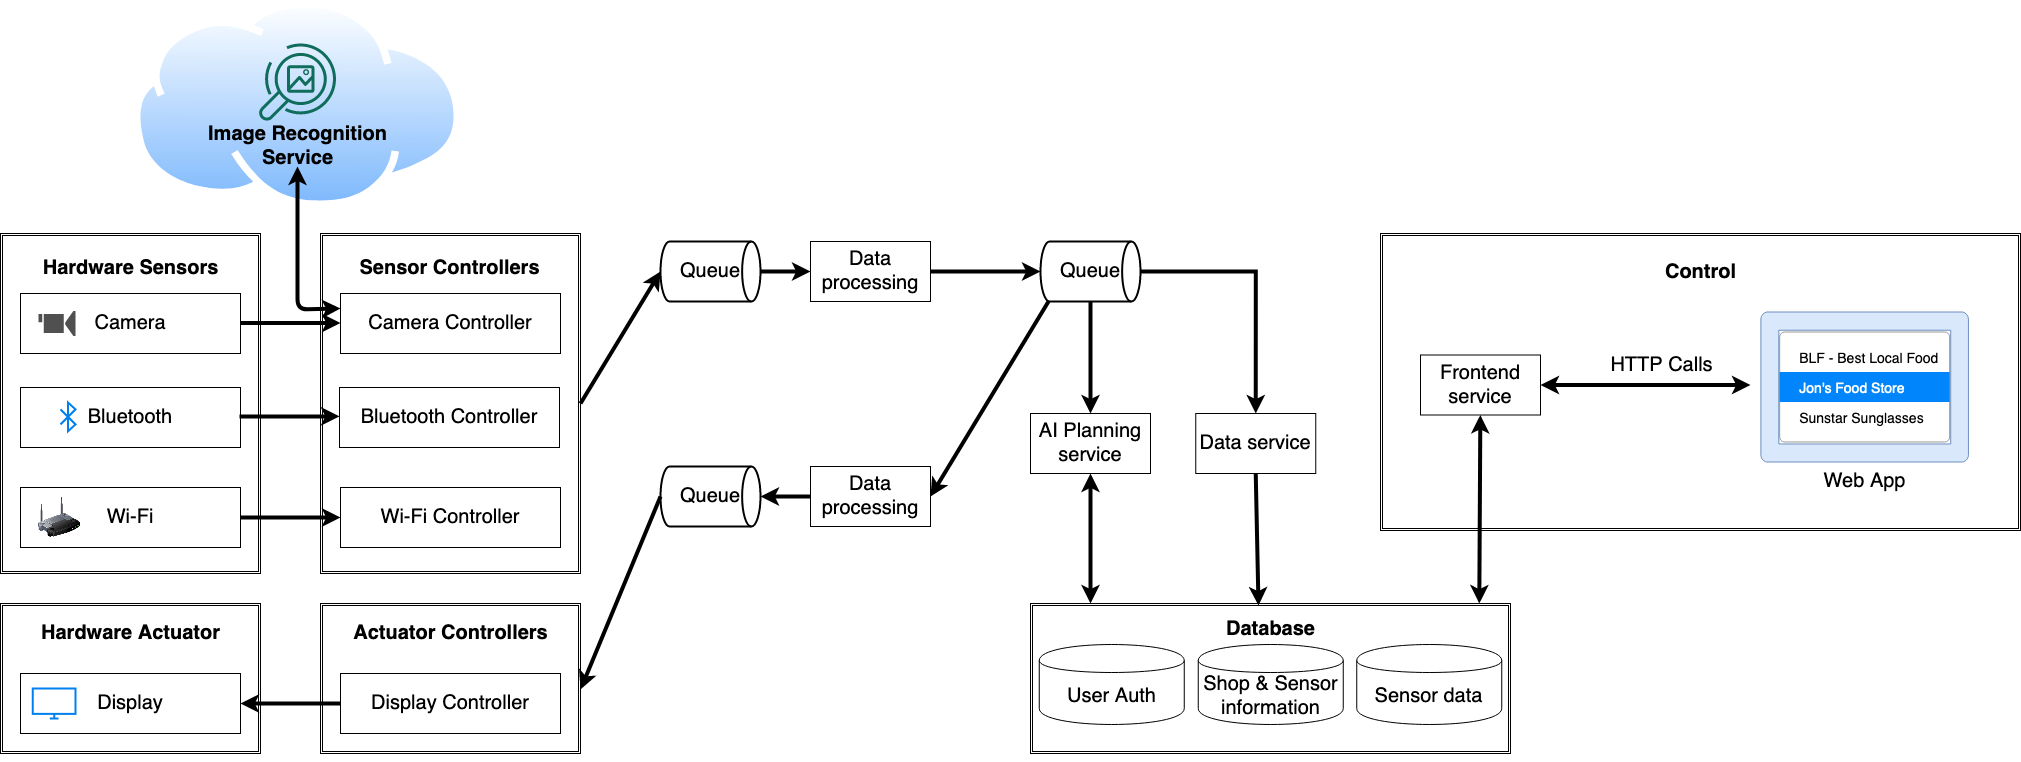
\includegraphics[width=\linewidth]{assets/architecture/Architecture.png}
    \caption{Overview of the system architecture}
    \label{fig:architecture}
\end{figure}

\section{System Implementation}\label{sec:implementation}
This section gives an in-depth explanation of the implementation of the guidance system. The implementation can be found on \url{https://github.com/seedrix/SmartCities/}. A quick overview of the main system components is given in section \ref{sec:architecture}. In the following the used tools and the implementation details of each system component, as well, as the communication mechanisms are described.

\subsection{Communication}\label{sec:conmunication}
For the implementation of the message queues of the system we used the Message Queuing Telemetry Transport (MQTT)\footnote{\url{https://mqtt.org/}} protocol. MQTT provides lightweight publish and subscribe messaging transport, optimized for high-latency and unreliable networks. To enable a fast development process, we used a public MQTT broker hosted by HiveMQ\footnote{\url{https://www.hivemq.com/public-mqtt-broker/}}. In order to run our system in production, a private MQTT broker should be hosted. 

To enable the communication between the web app and our system, an HTTP REST API is exposed by the frontend service. A detailed description of this API can be found in \cref{sec:frontendService}.

\begin{figure}

\dirtree{%
.1 de/smartcity/2020/mymall.
	.2 sensors.
		.3 ble.
			.4 <sensor id>.
				.5 count.
				.5 list.
			.4 \dots.
		.3 cam.
			.4 <sensor id>.
				.5 count.
			.4 \dots.
		.3 wifi.
			.4 <sensor id>.
				.5 count.
				.5 list.
			.4 \dots.
	.2 shops.
		.3 <shop id>.
		    .4 actuators.
		        .5 display.
		            .6 action.
			.4 people.
				.5 count.
			.4 sensors.
				.5 ble.
					.6 count.
					.6 list.
				.5 cam.
					.6 count.
				.5 wifi.
					.6 count.
					.6 list.
			.4 sensors\_raw.
				.5 ble.
					.6 <sensor id>.
						.7 count. 
						.7 list.
					.6 \dots.
				.5 \dots.
		.3 \dots.
}
\caption{MQTT topic hierarchy}
\label{fig:mqtt-topics}
\end{figure}


\subsection{Sensors}\label{sec:sensors}
To detect people, we used different types of sensors.
Every sensor has a unique id, which is used to match the sensor with the shop it belongs to. The sensors publish their data into MQTT topics and all data is encoded as JSON. The topic path for each sensor is determined by its id. Every sensor publishes its data into some topic below \topicname{/sensors/\{sensor id\}/}, which is referenced as the sensor's topic in the following. An overview of all used topics is shown in \cref{fig:mqtt-topics}. Analogously, also every shop has its own path in the topic hierarchy determined by its id: \topicname{/shops/\{shop id\}/}.


\subsubsection{BLE Sensors}
\label{impl:ble-sensor}
Since most modern smartphones are able to communicate via Bluetooth low energy and most people carry a smartphone with them, we use these signals to detect people at the shops. Usually, devices only send signals, if they want to communicate with other devices. 
In our scenario, these other devices would be most likely smartwatches or headphones. So per default, we could not assume, that any customer is wearing a smartwatch or headphones.
Just in time, Google and Apple released the Exposure Notification Framework\footnote{\url{https://www.apple.com/covid19/contacttracing}} for contact tracing. The protocol broadcasts periodically an id, which is changed every 15 minutes on average\footnote{\url{https://covid19-static.cdn-apple.com/applications/covid19/current/static/contact-tracing/pdf/ExposureNotification-BluetoothSpecificationv1.2.pdf}}, via Bluetooth low energy. Since the protocol communicates via Bluetooth low energy, we implemented our sensor to use these signals from the Exposure Notification Framework.
Our BLE Sensor is designed to run on a Raspberry Pi with BLE capability as a python script. In python, we use the bluepy\footnote{\url{https://github.com/IanHarvey/bluepy}} library to interface with the Bluetooth hardware. Since the Exposure Notification protocol was just released, there are no libraries to interact with it. Therefore, we implemented a parser by our self.
In our python script, we first wait some time to receive the signals. If a signal is received, we extract the ID and add it to a set. After the scanning period, the recorded IDs are hashed for privacy reasons and published via MQTT. Afterward, the set is cleared and we start with the scanning again. We use a scanning period of 30 seconds.
The data is published in two ways. The count of the elements in the set is published to the sensors \topicname{./count} topic.
Secondly, the list with the hashed IDs is published to the sensors \topicname{./list} topic. We use this list in a post-processing step to remove duplicates (see \cref{impl:ble-aggr}).
The ID of a BLE sensor starts with the letter 'b' followed by the mac address of the Bluetooth interface, so each BLE sensor uses a unique ID.
In \cref{fig:preprocessing_example} you can see an example of the payload of the \topicname{./list} topic.

\subsubsection{Cam Sensors}
\label{impl:cam-sensor}
Due to security reasons, cameras are omnipresent in shopping malls. They record the customers of the shops and cover nearly the whole shop area.
We want to utilize the already existing security camera systems to detect and count people. To extract information from the video footage, we use an image recognition approach to recognize people in the video footage. In order to keep the effort low and develop a prototype quickly, we used the cloud service Amazon Rekogniton\footnote{\url{https://aws.amazon.com/rekognition}} for the image recognition task. Furthermore, this ensures accurate results in a scalable manner.
The basic idea of this sensor is to extract single pictures from the video footage of the cameras in a predefined interval. Afterward, the pictures are sent to the AWS Rekognition service to label and count the people. 
To increase the simplicity when deploying our system in a real environment, our sensor takes all images into account that are placed in a certain folder. The only modification needed for an existing camera system is a script that periodically extracts images from the video stream of the camera and stores them in the folder of our sensor.
When the sensor detects a new image in the folder, it uploads the image to Amazon S3\footnote{\url{https://aws.amazon.com/s3/}} and then triggers the Amazon Rekogniton service to label the picture. Our sensor receives the resulting labels and extracts the people count from the result. This data is then published in the topic \topicname{/sensors/cam/\{some sensor id\}/count}.


\subsubsection{WiFi Sensors}
\label{impl:wifi-sensor}
Many shopping malls provide free WiFi to their customers. Also, the customers require an internet connection for their phones, to be able to interact with our web app. In our approach, we used a Raspberry Pi to act as an access point to which the customers can connect to. For this, we used the software RaspAP\footnote{\url{https://raspap.com}}. RaspAP provides an easy administration interface to set things up. In our configuration, each Pi serves as a DHCP server to assign IP addresses from a unique pool to the WiFi clients. 
%The software uses a file to keep track of which IP is assigned to which WiFi client.
Our python script uses shell commands to periodically extract a list of the connected WiFi clients. For this period, we used 30 seconds. The extracted data is published in two ways: The number of connected clients is published to the sensors \topicname{./count} topic. Since the MAC address of a device is unique, we can use it to identify a client across multiple access points. To increase the privacy of the customers, we are using the hashed value of the MAC address for further processing. We generate a map with the device IP addresses as keys and the hashed MACs as values and publish this map to sensors \topicname{./list} topic. We use this map in the later processing to remove duplicates (see \cref{impl:wifi-aggr}) in the case that a device switched to another AP inside the shop. 
Moreover, this data allows us to implement a mapping from a WiFi client to a user's account, so we could locate users across the mall. However, this remains for future work (see \cref{sec:discussion}).
The ID of a WiFi sensor starts with the letter 'w' followed by the mac address of the WiFi interface which is used for the AP. Therefore, each WiFi sensor uses a unique ID.
In this approach, we can only detect phones which are connected to our WiFi AP. There are alternative ways that work without the requirement that the customer must connect their phone to our AP. One approach is described by Georgievska et al.~\cite{Georgievska2019}.


\subsection{Sensor Data Processing}
\label{impl:sensor-processing}
The raw sensor data from each sensor is not very meaningful by itself. Therefore, we do some post-processing to the sensor data to add context and aggregate the values from multiple sensors to one value of a virtual sensor. All components described in this section are written in python and communicate only via MQTT with each other. This increases the flexibility and the loose-coupling of the system since each component could easily be swapped out and other components would be able to get data at any processing step in the processing pipeline. An overview of the post-processing steps is shown in \cref{fig:preprocessing}. At the first stage, the sensor data is enhanced with the information to which shop the sensor belongs to. This is done by the \componentname{ShopMapper} component. In the second stage, the data is aggregated for each shop and sensor type to a virtual sensor, e.g. data from all BLE sensors of one shop is combined to one overall virtual BLE sensor value for this shop. This is done by the respective \componentname{Aggregator} component for the sensor type. In the third stage, we combine the values for all sensor types per shop to calculate one value for the virtual people sensor which represents the estimated people at this shop. This is done by the \componentname{PeopleAggregator} component.


\subsubsection{Sensor Shop Mapping}
The \componentname{ShopMapper} component is subscribed to the general \topicname{/sensors/} topic and redirects the messages from the sensors to the corresponding shops. To achieve this, the \componentname{Shop\-Mapper} retrieves information about all shops from the database at startup. A mapping in which sensors and shops correspond to each other can be extracted from this data. Concretely, every message to the \topicname{/sensors/ble/\{some sensor id\}/list} topic would be published to the \topicname{/shops/\{some shop id\}/sensors\_raw\allowbreak/ble/\{some sensor id\}/list} topic of the appropriate shop in which the sensor is located. This is done analogously for the WiFi and cam sensors and the \topicname{count} topic. Additionally, the message payload is enhanced with a \attribute{shop\_id} attribute to ease to further processing. \cref{fig:preprocessing_example} shows an example with payloads.

\subsubsection{BLE Sensor Data Aggregation}
\label{impl:ble-aggr}
The \componentname{Ble\-Aggregator} component combines the data from all BLE sensors per shop and acts as a virtual BLE sensor per shop. It is subscribed to \topicname{/shops/+/sensors\_raw\allowbreak/ble/+/list}, so one instance of the component can handle the BLE sensors of all shops. The \componentname{Ble\-Aggregator} stores the last received message from all BLE sensors per shop. If a new message is received, the data of the messages is aggregated and published into the \topicname{/shops/\{some shop id\}/sensors/ble/count} and \topicname{/shops/\{some shop id\}/sensors/ble/list} topics of the shop. Since the Bluetooth signal of a device could be received by multiple sensors, duplicates can appear in the recorded IDs. To tackle this issue, we add all distinct IDs to a set and publish it to the \topicname{ble/list} topic. Afterward, the number of elements in the set is published to the \topicname{ble/count} topic. \cref{fig:preprocessing_example} shows an example with some payloads.

\subsubsection{Cam Sensor Data Aggregation}
\label{impl:cam-aggr}
The \componentname{CamAggregator} component combines the data from all cam sensors per shop and acts as a virtual cam sensor per shop. It is subscribed to \topicname{/shops/+/sensors\_raw\allowbreak/cam/+/count}. It sums up the counts from the cameras of a shop and publishes the result to \topicname{/shops/\{some shop id\}\allowbreak/sensors/cam/count}. 
%We use here only the count topic since we could not reference people across multiple cameras without implementing machine learning methods like face recognition. 
\begin{figure}
    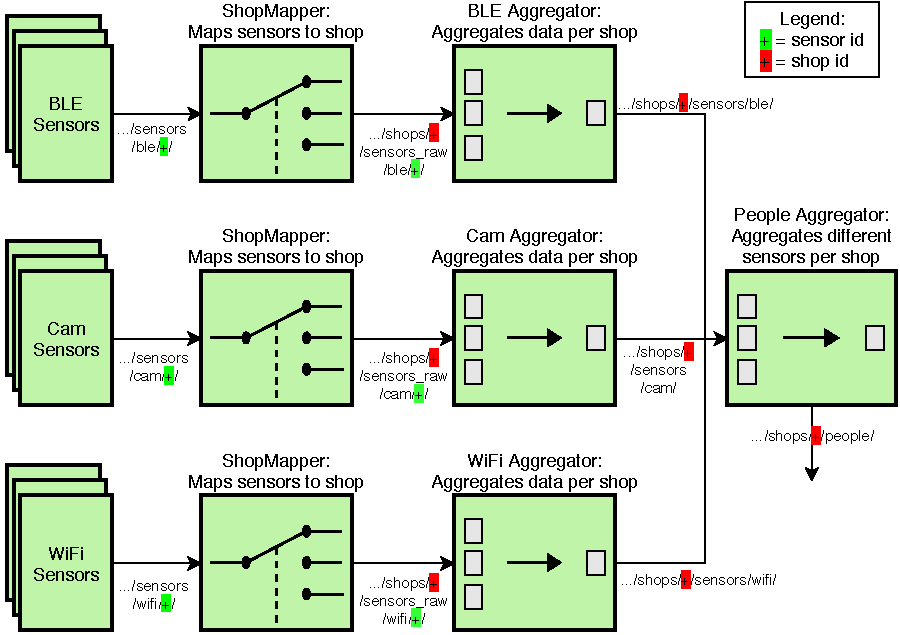
\includegraphics[width=.99\linewidth]{assets/sensor/sensor_preprocessing_overview_topics_small.pdf}
    \caption{Sensor data post-processing}
    \label{fig:preprocessing}
\end{figure}
\subsubsection{WiFi Sensor Data Aggregation}
\label{impl:wifi-aggr}
The \componentname{WiFiAggregator} component is very similar to the \componentname{Ble\-Aggregator} component and acts as a virtual WiFi sensor per shop. It is subscribed to \topicname{/shops/+\allowbreak/sensors\_raw\allowbreak/wifi\allowbreak/+/list}. The main difference is that the \componentname{WiFi\-Aggregator} works on maps instead of lists. It aggregates the maps in a way that every value in the resulting map is unique. This treats the case that a device was recorded by multiple sensors which can happen if the device switched between access points inside a shop.


\subsubsection{Sensor Data Aggregation per Shop}
\label{impl:people-aggr}
The \componentname{PeopleAggregator} component combines the data of the BLE, camera, and WiFi data per shop. So it acts as the virtual people sensor per shop. It is subscribed to \topicname{/shops/+/sensors\allowbreak/+/count} and calculates the mean of the count-values from all the sensor types of the shop. This value is published to \topicname{/shops/\{some shop id\}\allowbreak/people/count}.
\cref{fig:preprocessing_example} shows an example with a message to this topic. To ease the monitoring, this message also contains information about the number and types of the aggregated sensors used to calculate the value.

\begin{figure}
    \centering
    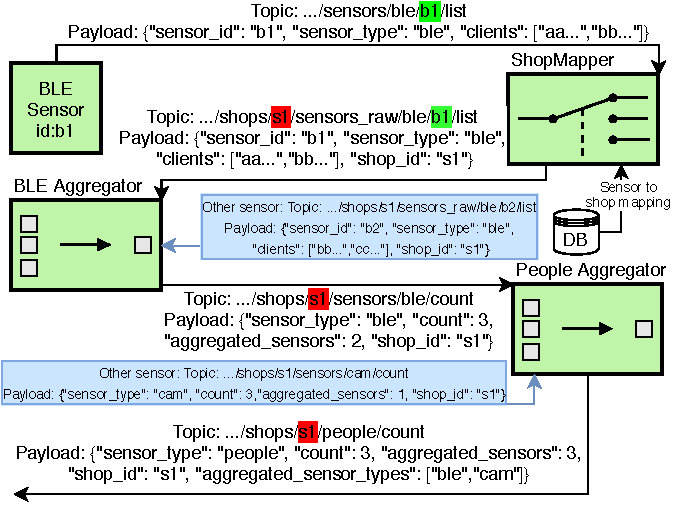
\includegraphics[width=0.9\linewidth]{assets/sensor/preprocessing_ble_payload.pdf}
    \caption{Example message flow of BLE sensor data processing with message payloads}
    \label{fig:preprocessing_example}
\end{figure}

\subsection{AI Planning}\label{sec:ai}
The AI planning service is the core of our system. It computes plans for all customers such that the people are evenly distributed among the shops in the shopping mall regarding the capacities of each shop and the requests of the customers. As the AI planning solver we use Metric-FF\footnote{\url{https://fai.cs.uni-saarland.de/hoffmann/metric-ff.html}} which is an extension of the FF\footnote{\url{https://fai.cs.uni-saarland.de/hoffmann/ff.html}} planner to support numerical functionality. We chose this solver because it supports level 2 of the PDDL description~\cite{hoffmann2003metric}. This is required for our system because for the distribution of the customers we need to be able to compare numerical values in the PDDL problem file. Furthermore, Metric-FF is highly performant~\cite{hoffmann2003metric}. 

The AI planning service queries periodically the users' shop preferences and current and maximum shop utilization from the database and starts the AI planner on this data. Afterward, the next shop attribute of each user is updated in the database accordingly to the decision of the planner.

\subsubsection{Domain File}
Listing \ref{lst:pddl} shows the PDDL problem file. We have the objects list and shop. A list describes the shops a customer wants to visit and is associated with a user. At-shop is the predicate that describes the recommendation for the next shop the customer should visit. This is the main part of the computed plan. The predicate list-set describes if a shop is chosen for a specific list. At the end of the computation, each list has to have an associated shop. Shop-option describes the shop preferences of the user. For each selected shop of a user, there is a shop-option combining this user and the shop. The action choose determines a shop for a user. This action is not possible if for this user a shop is already chosen or if the shop is not one of the user's preferences. The effect of this action is that the predicates list-set and at-shop are set accordingly as well as the function people-at-shop for the chosen shop is increased by one.
\lstinputlisting[
  float=!htb,
  caption={PDDL problem file},
  label={lst:pddl},
  language=PDDL]
  {domain.pddl}

\subsubsection{Problem File}
The problem file has an object of type list for each active user who selected a list of requested shops he wants to visit. Moreover, the shops in the shopping mall are defined. The initial value for the function people-at-shop is set to the number of people the sensors captured in that shop (see \cref{sec:sensors}). The goal is that all list-set holds for all lists and the function people-at-shop is lower than a specified limit. This limit is initialized with the maximum number of people that can visit the shop at the same time. If the planning problem does not have a solution, the limit is increased iteratively until a solution is found. In this case, some customers must wait before they can visit a shop which is displayed by monitors in front of each shop (see \cref{sec:displays}). 

At first glance, the problem that needs to be solved might rather look easy to solve. However, trivial approaches like selecting one of the shops that are requested and have still capacity do not lead to the best solutions and are in general inaccurate. Solving the problem with AI planning and the described construction of the problem produces the optimal solution and has a high performance as long as the number of shops is not uncommonly high.


\subsection{Database}
We use a MongoDB\footnote{\url{https://www.mongodb.com/}} database for the persistent storage of our data.
We have three different types of data that we store in databases:
\begin{enumerate}
    \item The authentication data for user which contains the email and the hash value of the password
    \item The information about shops and sensors and the mapping between them
    \item Sensor data which is published over MQTT topics
\end{enumerate}

We use the data service component to automatically store MQTT messages from specific topics to our database.
This is relevant to provide access to historical data for other components of our system.
Our implementation is based on \url{https://github.com/David-Lor/MQTT2MongoDB}.

\subsection{Frontend Service}\label{sec:frontendService}
The frontend service exposes a REST API to interact with our system. To create the API, we used the framework Flask\footnote{\url{https://github.com/pallets/flask}} in combination with the extension Flask-RESTful\footnote{\url{https://github.com/flask-restful/flask-restful}}.

The frontend service is divided into three sub-APIs: Shops, User, and Auth. In the following, all three are described.
\subsubsection{Shops-API}

The Shops-API handles all requests regarding the information of the shops. 

\routes{/shops/all}{
    \method{GET}{
        \desc{Returns a list of all shops}
        \postcond{Content-Type: application/json}
        \statuscodes{\status{200} \sep \status{500}}
    }
}


\routes{/shops/shop/<string:shop_id>}{
    \method{GET}{
        \desc{Returns specific information for the requested shop.}
        \precond{\url{shop_id} is a valid ID for a shop in the database}
        \postcond{Content-Type: application/json}
        \statuscodes{\status{200} \sep \status{404} \sep \status{500}}
    }
    \method{PUT}{
        \desc{Creates or updates a shop}
        \precond{Content-Type: application/json \sep body contains a valid description of a shop}
        \body{\{
            "max\_people1" : 2,
            "sensors" : [ 
                "bB8:27:EB:2A:C9:E6", 
                "wb8:27:eb:d5:36:19", 
                "ccamera0"
            ],
            "shop\_name" : "BLF - Best Local Food",
            "logo" : "data:image/svg+xml;base64,PD94bW..."
        \}}
        \statuscodes{\status{200} \sep \status{400} \sep \status{500}}
    }
}

\routes{/shops/people/<string:shop_id>}{
    \method{GET}{
        \desc{Returns the current number of people at the requested shop}
        \precond{\url{shop_id} is a valid ID for a shop in the database}
        \postcond{Content-Type: application/json}
        \statuscodes{\status{200} \sep \status{404} \sep \status{500}}
    }
}

\routes{/shops/people/<string:shop_id>/<int:timestamp>}{
    \method{GET}{
        \desc{Returns all people data for the given shop after the requested timestamp}
        \precond{\url{shop_id} is a valid ID for a shop in the databas \sep \url{timestamp} is a valid unix time timestamp}
        \postcond{Content-Type: application/json}
        \statuscodes{\status{200} \sep \status{404} \sep \status{500}}
    }
}

\subsubsection{Auth-API}
The Auth-API handles user authentication. It enables the user to sign up and to log in to our application. For authentication purposes, a JSON Web Token (JWT) is generated. The whole state is included in the JWT which saves us to manage the authentication tokens on the server-side. The JWT expires after one day which is suitable for our use case.

\routes{/auth/signup}{
    \method{POST}{
        \desc{Creates a new user account with the given email and password}
        \precond{body contains an email and password \sep the email address is not already in use \sep Content-Type: application/json}
        \postcond{send JWT token \sep create user}
        \body{\{
        	"email": "test@email.com",
        	"password": "test1234"
        \}}
        \statuscodes{\status{200} \sep \status{400} \sep \status{500}}
    }
}

\routes{/auth/login}{
    \method{POST}{
        \desc{Log in a registerd user}
        \precond{body contains an email and password \sep the user exists in our database \sep email and password are correct \sep Content-Type: application/json}
        \postcond{send JWT token}
        \body{\{
        	"email": "test@email.com",
        	"password": "test1234"
        \}}
        \statuscodes{\status{200} \sep \status{400} \sep \status{500}}
    }
}

\subsubsection{User-API}
The User-API handles all user-specific tasks. A JWT must be attached to all requests to this API for authentication purposes.

\routes{/user/next_shop}{
    \method{GET}{
        \desc{Returns the recommended next shop for the user}
        \precond{JWT}
        \postcond{Content-Type: application/json}
        \statuscodes{\status{200} \sep \status{401} \sep \status{500}}
    }
}

\routes{/user/shops}{
    \method{GET}{
        \desc{Returns the list of selected shop for the user}
        \precond{JWT}
        \postcond{Content-Type: application/json}
        \statuscodes{\status{200} \sep \status{401} \sep \status{500}}
    }
    \method{PUT}{
        \desc{Sets the list of selected shops for the user }
        \precond{JWT \sep Content-Type: application/json \sep body contains valid list of shops}
        \body{[
            "shop1",
            "shop2"
        ]}
        \statuscodes{\status{200} \sep \status{401} \sep \status{500}}
    }
}

\routes{/user/shops/<string:shop_id>}{
    \method{DELETE}{
        \desc{Deletes the shop from the list of selected shop, if the shop was on the list}
        \precond{JWT}
        \statuscodes{\status{200} \sep \status{401} \sep \status{500}}
    }
}


\subsection{Frontend}
A web app is used to interact with our guidance system. Furthermore, users are notified which shop should be visited next. We used the Angular Framework\footnote{\url{https://angular.io/}} to implement our frontend. Additionally, our implementation uses Angular Material for the components design and MDBootstrap Free\footnote{\url{https://mdbootstrap.com/docs/angular/}} for chart
visualizations which is licensed under the MIT license\footnote{\url{https://mdbootstrap.com/general/license/}}. Using a component library leads to a consistent look of the user interface. The frontend gets the latest data by HTTP requests to the frontend service (see \cref{sec:frontendService}).
In the following, we describe the frontend and its functionality. The navigation is done with a side menu to increase the usability on mobile devices (see \cref{fig:sidenav}).

\begin{figure}
    \centering
    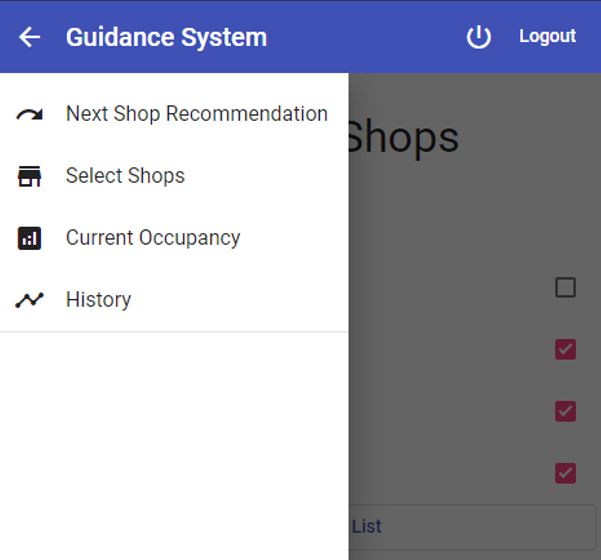
\includegraphics[width=0.6\textwidth]{assets/frontend/sidenav.png}
    \caption{Side menu}
    \label{fig:sidenav}
\end{figure}

\subsubsection{User Management}
The web app contains a user management. Users can sign up and log in to their accounts by specifying their e-mail address and a password (see \cref{fig:login}). The form automatically checks if the given input is syntactically valid. The authentication is done with a bearer token\footnote{https://oauth.net/2/bearer-tokens/}. The token is returned from the frontend service and saved in the local browser storage. HTTP-Requests that are sent to the backend are then complemented with the token. The user management enables the use of the application on several devices.
\begin{figure}
    \centering
    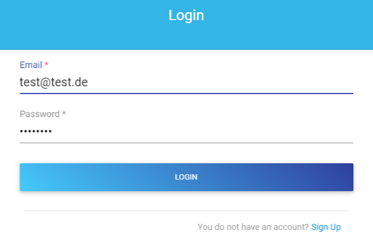
\includegraphics[width=0.6\textwidth]{assets/frontend/login.png}
    \caption{Login page}
    \label{fig:login}
\end{figure}

\subsubsection{Shop Selection}
The frontend contains a page that shows all shops in the shopping mall and allows the user to select a subset that he wants to visit during his purchase at the mall. The data is sent to the frontend service with an HTTP-Post message. Afterward, the recommended shop for the user that is computed with the AI planner (see \cref{sec:ai}) considering the user lists, as well as the current occupancy rates are shown.   

\subsubsection{Data Visualization}
The database contains the number of customers at each shop. This occupancy rate can be displayed in a bar chart for each shop next to the maximum number of customers for that shop. Furthermore, the historical data can be shown in a line chart (see \cref{fig:history}). This is useful for customers to analyze the times at which the shopping mall in general or the shops they want to visit are less frequented and to avoid crowds of customers, therefore. 


\begin{figure}
    \centering
    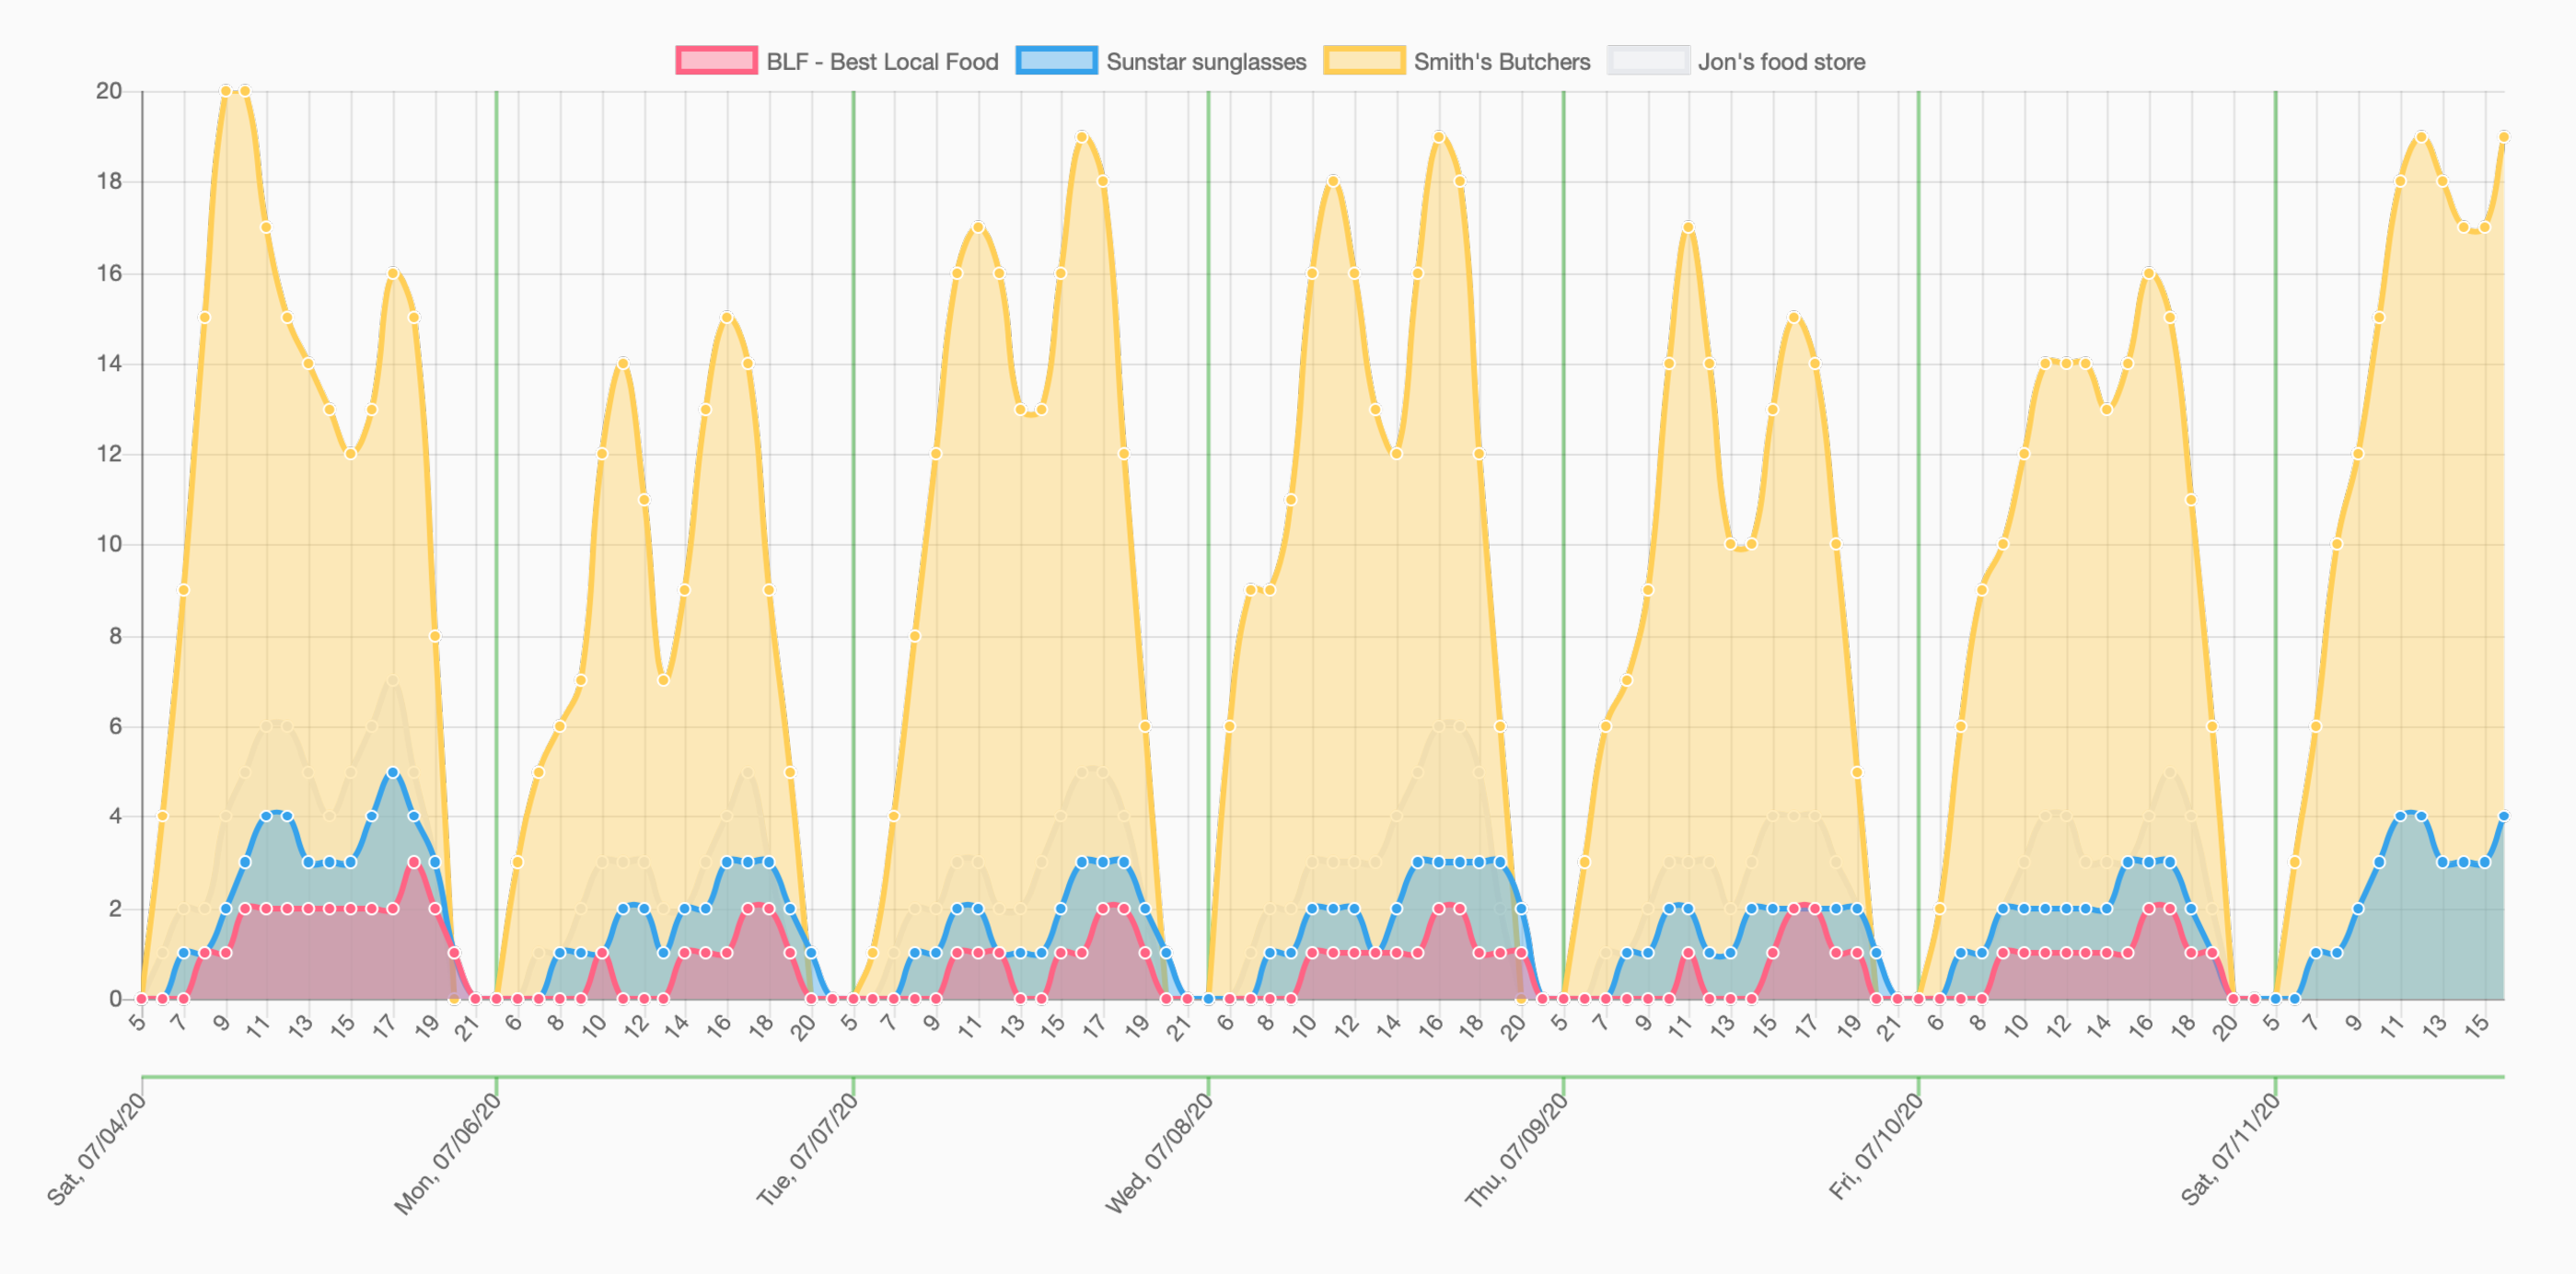
\includegraphics[width=1\textwidth]{assets/frontend/history.pdf}
    \caption{Visualization of the history for one week}
    \label{fig:history}
\end{figure}


\subsection{Displays}\label{sec:displays}
The \componentname{ShopDisplay} components are used to control the number of people in the shops. A \componentname{ShopDisplay} is a display in front of the shop which shows to the customer if he is allowed to enter the shop or not. We implemented the shop displays as an HTML page. The page connects via WebSocket to the MQTT broker and subscribes to the \topicname{actuators/display/action} topic of the particular shop. The page is stateless and the shop is set via the URI fragment. For example, the page \topicname{display.html\#shop1} will subscribe to the topic \topicname{/shops/shop1/actuators\allowbreak/display/action}. The JSON messages in this topic contain the following attributes: \attribute{symbol}, \attribute{color} and \attribute{message}. \attribute{color} defines the background color of the page, \attribute{message} contains the message which should be displayed, and \attribute{symbol} contains a base64 encoded image, which will be displayed below the message text. This allows us to display highly customizable messages to the customers. In fact, the message attribute could also contain HTML content which would be rendered on the page.

\subsubsection{Display Controller}\label{sec:display-control}
The \componentname{DisplayController} component is used to control the \componentname{ShopDisplay}. The \componentname{DisplayController} retrieves the maximum number of allowed people per shop from the database and listens to the \topicname{people/count} topic of the shops. If the people count is above 95\% of the maximum shop capacity, the \componentname{DisplayController} will publish a message with the message text "Don't enter! Please wait", red background and an appropriate symbol to the \topicname{/shops/\{some shop id\}/actuators\allowbreak/display/action} topic of the shop. If the utilized capacity is below this threshold, it will publish a message to this topic, which will encourage the customers to enter the shop.

\subsection{Test Data Generation}
Since we do not operate a shopping mall, we are not able to record real data to test the system. In order to tackle this issue, we implemented two ways of data generation: Live sensor data and historical sensor data. To generate live sensor data, we implemented a dashboard that acts as simulated sensors and provides some simple monitoring features. To obtain historical data, we wrote a script to extract data from Google's \textit{Popular times} feature and insert it into our database.

\subsubsection{Simulated Sensors}
To test the system without the need of a bunch of Raspberry Pis and real people, we wrote a sensor dashboard where we can set the values of simulated sensors for each shop. Also, it provides us with monitoring features that are helpful for debugging. The dashboard is written as a web app with HTML and JavaScript. It uses MQTT to publish sensor data to the sensor topics like the real sensors would do. The values can be set manually or be copied from an array of values with some delay to simulate sensors over time. Additionally, the dashboard shows the values of our virtual aggregated sensors per shop.

\subsubsection{Historical Test Data}
To gather historical data, we used data from Google Maps' \textit{Popular times}\footnote{\url{https://support.google.com/business/answer/6263531?hl=en}} feature. This feature shows how busy a particular shop is per hour and weekday. In order to extract this data, we wrote a JavaScript snippet to gather the HTML data of the page. A python script then uses this data and maps it to the capacity of a shop and writes it to our database in the same way the data of the virtual people sensor would be written to the database.

%Describe the implementation of your system. This section is only relevant for the report and should be %omitted for the project description. 

\section{Discussion and Conclusions}\label{sec:discussion}
The implemented guidance system can be used to guide customers in a shopping mall with the goal to distribute them equally among the individual shops. This results in less waiting time for the customers as well as less crowding in the shops. The system is highly scalable and fault-tolerant due to the usage of the messaging protocol MQTT. Moreover, our responsive web app ensures usability.

Future work is the improvement of the accuracy of the sensors by using machine learning. In this context, the various sensors can be trained with annotated data from the environment in which the system runs. This can increase the accuracy of the people estimations. Another aspect of future work is to extend the planning service to consider historical data to improve the recommendations. Furthermore, 
this would allow us to give guiding recommendations for the future. Instead of suggesting only the next shop a user should visit, the system could output a list of shops. Additionally, the mapping from WIFI clients to users could be used to track the users automatically. This could be used to increase the usability of the system because the input that a user left a shop could be omitted in this case.
To conclude, one can say that our system shows the feasibility and the usefulness of a guidance system in shopping malls.
%
% ---- Bibliography ----
%
\bibliographystyle{splncs04}
\bibliography{mybib}

All links were last followed on July 11, 2020.

\end{document}